\documentclass[11pt,letterpaper]{article}

%\usepackage{fontspec}
%\usepackage[utf8]{inputenc}
\usepackage{textcomp,marvosym}
\usepackage{amsmath,amssymb}
\usepackage[normalem]{ulem}
\usepackage[left]{lineno}
\usepackage{changepage}
\usepackage{sidecap}
\usepackage{rotating}
\usepackage{color}
\usepackage{natbib}
\usepackage{setspace}
\usepackage{}
\usepackage{fancyhdr}
\usepackage{graphicx}
\usepackage{xspace}
\usepackage{threeparttable}
\usepackage{color,colortbl}
\usepackage{url}
%\usepackage[hidelinks]{hyperref}
\urlstyle{same}
\doublespacing

\raggedright
\textwidth = 6.5 in
\textheight = 8.25 in
\oddsidemargin = 0.0 in
\evensidemargin = 0.0 in
\topmargin = 0.0 in
\headheight = 0.0 in
\headsep = 0.5 in
\parskip = 0.1 in
\parindent = 0.1in

% Bold the 'Figure #' in the caption and separate it from the title/caption with a period
% Captions will be left justified
\usepackage[aboveskip=1pt,labelfont=bf,labelsep=period,justification=raggedright,singlelinecheck=off]{caption}

% Remove brackets from numbering in List of References
%\makeatletter
%\renewcommand{\@biblabel}[1]{\quad#1.}
%\makeatother

% Self defined commands
\newcommand{\degreesC}{\textdegree C\xspace}
\newcommand{\degrees}{\textdegree\xspace}
\newcommand{\dC}{$\delta^{13}$C\xspace}
\newcommand{\dO}{$\delta^{18}$O\xspace}
\newcommand{\SrSr}{$^{87}$Sr/$^{86}$Sr\xspace}
\newcommand{\permil}{\textperthousand\xspace}
\newcommand{\UPb}{$^{206}$Pb/$^{238}$U\xspace}
\newcommand{\pCOtwo}{\textit{p}CO$_{2}$\xspace}
\newcommand{\COtwo}{CO$_{2}$\xspace}
%

\setcounter{figure}{0}
\renewcommand{\thefigure}{SI\arabic{figure}}
\setcounter{table}{0}
\renewcommand{\thetable}{SI\arabic{table}}

\definecolor{Yellow}{rgb}{1,1,0.35}
%

\pagestyle{myheadings}
\pagestyle{fancy}
\fancyhf{}
\lhead{Park et al., in preparation}
\rhead{\thepage}

\begin{document}

\begin{flushleft}
{\Large \textbf{Supplementary Information for ``Emergence of Indonesia and New Guinea as a driver for Neogene cooling''}}

Yuem Park\textsuperscript{1},
Pierre Maffre\textsuperscript{1},
Nicholas L. Swanson-Hysell\textsuperscript{1},
Francis A. Macdonald\textsuperscript{2},
Eliel A. Anttila\textsuperscript{2},
Yves Godd\'eris\textsuperscript{3}

\bigskip
\textsuperscript{1} Department of Earth and Planetary Science, University of California, Berkeley, CA, USA

\textsuperscript{2} Department of Earth Science, University of California, Santa Barbara, CA, USA

\textsuperscript{3} G\'eosciences Environnement Toulouse, CNRS--Universit\'e Paul Sabatier - IRD, Toulouse, France

\bigskip

\end{flushleft}

\linenumbers

These supplementary information materials provide details on the model framework used in this study. Code associated with this study can be found at: \url{https://github.com/Swanson-Hysell-Group/XXX}.

\section*{Silicate Weathering Component}

\begin{SCfigure}[0.6][h!]
\begin{center}
	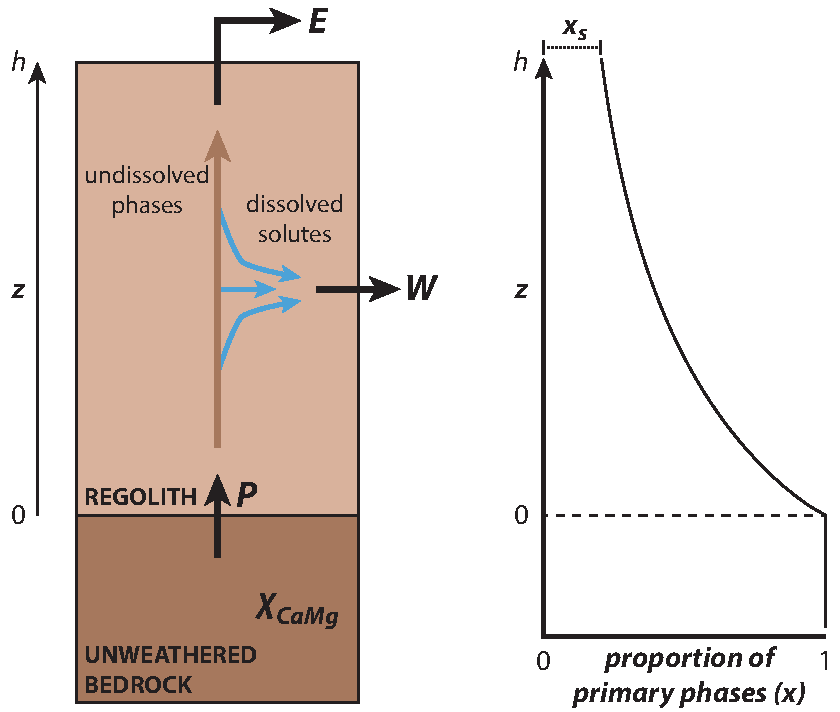
\includegraphics[width=0.6\textwidth]{../Figures/regolith_schematic.pdf}
	\caption{A schematic representation of the silicate weathering component of GEOCLIM in a single profile at steady-state. A rock particle leaves the unweathered bedrock with production rate $P_{r}$, and transits vertically through a regolith of height $h$. Regolith production and physical erosion ($E_{p}$) are equal at steady-state. As the particle transits upwards, some fraction of the primary phases ($x$) are chemically weathered ($W$) with the flux of Ca and Mg corresponding to that weathering rate multiplied by the concentration of Ca+Mg in unweathered bedrock ($\chi_{CaMg}$).}
	\label{fig:regolith_schematic}
\end{center}
\end{SCfigure}

The silicate weathering component of the GEOCLIM model has been improved compared to the previously published version \citep{Godderis2017b}. The new component implements the model of \cite{Gabet2009a} for the development of a chemically weathered profile. We refer to this chemically weathered profile as regolith where the base of the regolith is unweathered bedrock. In the model of \citet{Gabet2009a}, material enters the regolith and leaves either as a solute through chemical weathering of the material during its travel from the bedrock towards the surface, or as a physically weathered particle once it reaches the top. We use the DynSoil implementation of the \cite{Gabet2009a} model which integrates a climatic dependence on the chemical weathering that occurs within the regolith using the formulation of \cite{West2012a}. The transient time-varying version of this regolith model is described by the following system of three equations which form the core of the new DynSoil component of GEOCLIM:

\begin{equation}
    \frac{dh}{dt} = P_{r} - E_{p}
    \label{eq:1}
\end{equation}

\begin{equation}
    \frac{\partial x}{\partial t} = -P_{r} \frac{\partial x}{\partial z} - K \tau^{\sigma}x
    \label{eq:2}
\end{equation}

\begin{equation}
    \frac{\partial \tau}{\partial t} = -P_{r} \frac{\partial \tau}{\partial z} + 1
    \label{eq:3}
\end{equation}

\noindent
Equation \ref{eq:1} is a statement of material conservation, where $h$ is the total height of the regolith (m), $t$ is the model time (yr), $P_{r}$ is the regolith production rate (m/yr), and $E_{p}$ is the physical erosion rate (m/yr). Equation \ref{eq:2} describes how the residual fraction of weatherable phases ($x$, unitless) changes as a function of time ($t$, yr) and depth (where $z$ is the height above the base of the regolith; m). $K \tau^{\sigma}$ is the dissolution rate constant, which depends on the local climate (captured by $K$, yr$^{-1-\sigma}$) and the time that a given rock particle has spent in the regolith ($\tau$, yr) to some power $\sigma$ (unitless) which implements a time-dependence. Equation \ref{eq:3} describes how the time that a given rock particle has spent in the regolith changes as time in the model progresses.

The net weathering rate in the regolith column ($W$, m/yr) can then be calculated with:

\begin{equation}
    W = \int_{0}^{h} K \tau^{\sigma} x\;dz
    \label{eq:4}
\end{equation}

The regolith production rate can be expressed as the product of the optimal production rate ($P_{0}$) and a soil production function ($f(h)$):

\begin{equation}
    P_{r} = P_{0}\;f(h)
    \label{eq:5}
\end{equation}

\begin{equation}
    P_{0} = k_{rp}\;q\;e^{-\frac{E_{a}}{R}\left(\frac{1}{T}-\frac{1}{T_{0}}\right)}
    \label{eq:6}
\end{equation}

\begin{equation}
    f(h) = e^{-\frac{-h}{d_{0}}}
    \label{eq:7}
\end{equation}

\noindent
$P_{0}$ is the `optimal' regolith production rate (m/yr), which is defined to be the regolith production rate when there is no overlying regolith. In Equation \ref{eq:6}, we parameterize this value using the model of \citet{Carretier2014a}, where $k_{rp}$ is a proportionality constant (unitless), $q$ is the runoff (m/yr), $E_{a}$ is the activation energy (J/K/mol), $R$ is the ideal gas constant (J/mol), $T$ is the temperature (K), and $T_{0}$ is the reference temperature (K). $f(h)$ is the soil production function (unitless), which describes how regolith production decreases as the thickness of the regolith increases. It takes an exponential form as is commonly applied in the literature (e.g. \citealp{Gabet2009a}). In Equation \ref{eq:7}, we follow \citet{Heimsath1997a}, where $d_{0}$ is a reference regolith thickness (m).

Our implementation of the erosion rate follows one of the approaches taken in \citet{Godderis2017c} and \citet{Maffre2018a}, where it is parameterized based on runoff and slope ($s$; m/m):

\begin{equation}
    E_{p} = k_{e}\;q^{m}\;s^{n}
    \label{eq:8}
\end{equation}

\noindent
$k_{e}$ is a proportionality constant ((m/yr)$^{1-m}$) and $m$ and $n$ are adjustable exponents that are kept as 0.5 and 1 as in \citet{Maffre2018a}. This formulation is close to the large-scale BQART model of \citet{Syvitski2007a}, but without a temperature dependence and the replacement of elevation with slope, resulting in functional form that more closely resembles the stream power law \citep{Davy2000a}. This formulation and these exponent values are supported by various compilations (e.g. \citealp{Lague2013a}) although \citet{Lague2013a} also suggests that there is variability in the proportionality constant that is difficult to capture at a global scale.

The $K$ in the dissolution rate constant in Equation \ref{eq:2} describes the dependence of the chemical weathering on climate:

\begin{equation}
    K = k_{d}\left(1-e^{-k_{w}q}\right)e^{-\frac{E_{a}}{R}\left(\frac{1}{T}-\frac{1}{T_{0}}\right)}
    \label{eq:9}
\end{equation}

\noindent
Equation \ref{eq:9} is an empirical simplification of mineral dissolution rates derived from kinetic theory and laboratory experiments \citep{West2012a}, where $k_{d}$ is a proportionality constant that modifies the dependence of dissolution rate on runoff and temperature (yr$^{-1-\sigma}$), and $k_{w}$ is a proportionality constant that modifies the dependence of dissolution rate on runoff (yr/m).

In this study, we are interested in obtaining the steady-state solution rather than the transient time-varying solution. The steady-state solution for DynSoil can be calculated analytically by setting the time derivatives equal to zero resulting in the following set of equations:

\begin{equation}\label{eq:dynsoil_ss}
\left\{\ 
\begin{aligned}
& h   \ =\    \max\left(  \;  0  \;,\;  d_{0} \log\left(\frac{P_{0}}{E_{p}}\right)  \right)                                                 \\
& x(z)      \ =\   \exp\left(   - \frac{K}{\sigma+1}  \left(\frac{z}{E_{p}}\right)^{\sigma+1}   \right)   \\
& W        \ =\   (1-x(h)) \, E_{p}  \ =\   (1-x_s) \, E_{p}                                                                         \\
\end{aligned}
\right.
\end{equation}

\noindent
$x(z)$ is the abundance profile of primary phases inside the regolith, varying with height upward from the base of the regolith as shown in Figure \ref{fig:regolith_schematic}. Setting $z$ equal to the regolith thickness ($h$) gives $x_s$ which is the proportion of primary phases remaining at the top of the regolith column.

\section*{Implementation of Lithology}

\begin{table}[h!]
\begin{center}
\resizebox{0.7\textwidth}{!}{
    \begin{tabular}{cclcl}
    \textbf{GLiM} & \textbf{GLiM} & \textbf{GLiM} & \textbf{GEOCLIM} & \textbf{GEOCLIM}\\
    \textbf{ID} & \textbf{code} & \textbf{classification} & \textbf{ID} & \textbf{classification}\\
    &&&& \\
    \hline
    &&&& \\
    1 & su & unconsolidated sediments & 6 & sediments \\
    2 & vb & basic volcanic rocks & 4 & mafics \\
    3 & ss & siliciclastic sedimentary rocks & 6 & sediments \\
    4 & pb & basic plutonic rocks & 4 & mafics \\
    5 & sm & mixed sedimentary rocks & 6 & sediments \\
    6 & sc & carbonate sedimentary rocks & 5 & carbonates \\
    7 & va & acid volcanic rocks & 2 & felsics \\
    8 & mt & metamorphics & 1 & metamorphics \\
    9 & pa & acid plutonic rocks & 2 & felsics \\
    10 & vi & intermediate volcanic rocks & 3 & intermediates \\
    11 & wb & water bodies & 0 & water/ice \\
    12 & py & pyroclastics & 2 & felsics \\
    13 & pi & intermediate plutonic rocks & 3 & intermediates \\
    14 & ev & evaporites & 5 & carbonates \\
    15 & nd & no data & 1 & metamorphics \\
    16 & ig & ice and glaciers & 0 & water/ice \\
    \end{tabular}
}
\vspace{10pt}
\caption{Grouping of 16 lithologic categories in GLiM \citep{Hartmann2012a} to 6 broader categories for GEOCLIM.}
\label{tab:GLiM_to_GEOCLIM}
\end{center}
\end{table}

\begin{figure}[h!]
    \centering
    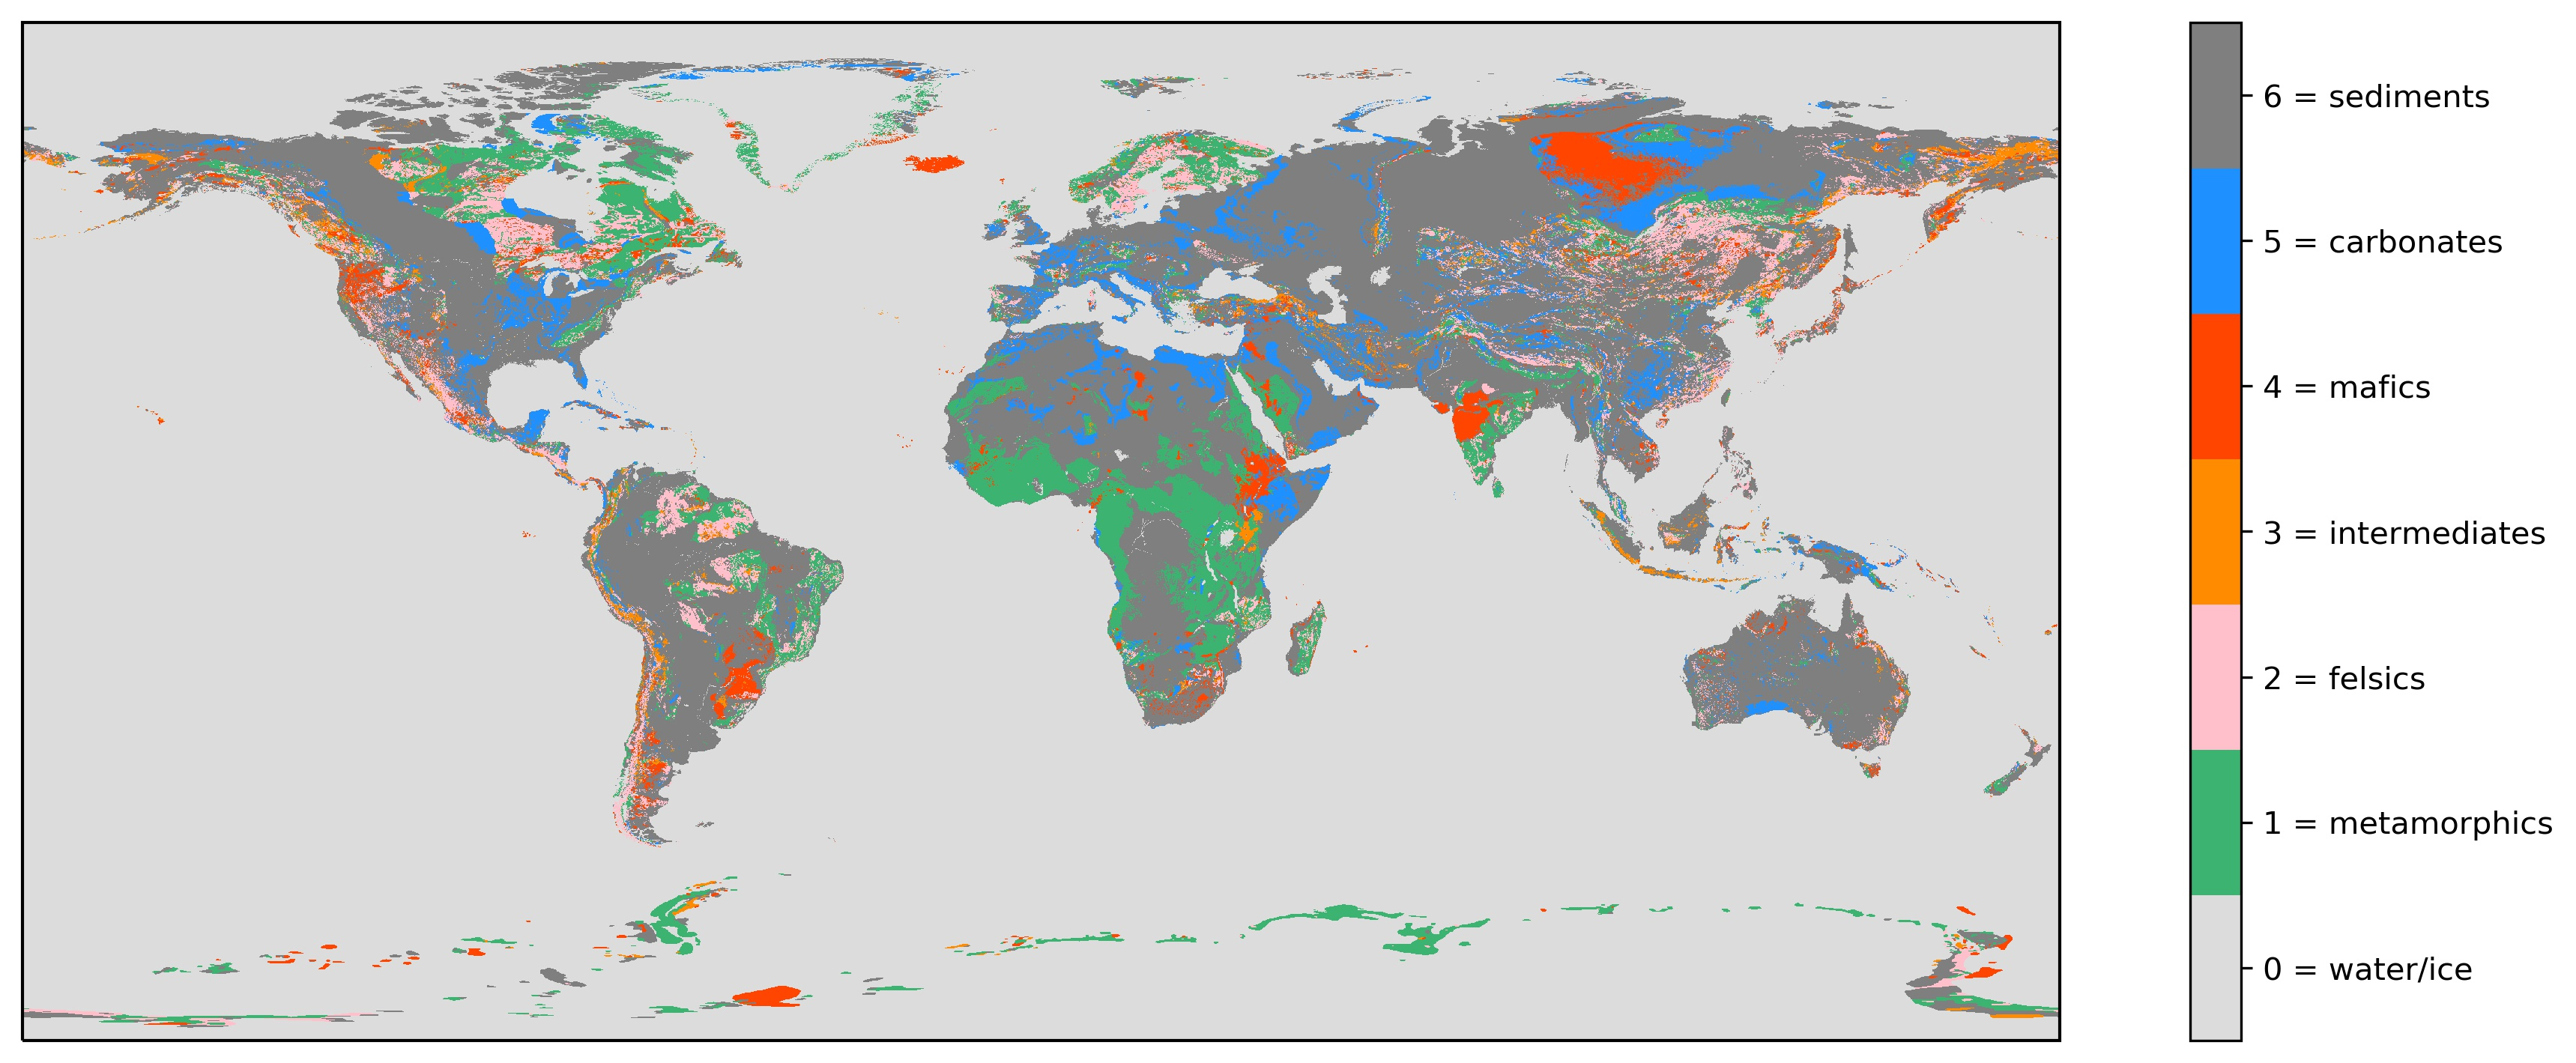
\includegraphics[width=1\textwidth]{Manuscript/Figures/world_lithology.jpg}
    \caption{Distribution of lithologies at 0.1\degrees $\times$ 0.1\degrees resolution used in GEOCLIM.}
    \label{fig:world_lithology}
\end{figure}

We restricted the calculation of the weathering fluxes to the flux of dissolved Ca+Mg originating from continental silicate weathering, as they are the sole contributors to the long-term consumption of atmospheric \COtwo. To calculate this flux, we need to assign the concentration of Ca and Mg ($\chi_{CaMg}$) within the unweathered bedrock (Fig. \ref{fig:regolith_schematic}). Previous implementations of GEOCLIM have used bulk continental crust values across all exposed land, using the concept of ``diffuse lithology'' (it was assumed that the weathering rates of all rocks was the same for each continental grid element, provided that the grid element was submitted to the same climatic conditions). Given that the hypothesis we seek to test involves the varying concentration of cations in different lithologies, the diffuse lithology cannot be used anymore, and instead we have implemented a more realistic lithologically-resolved version of the model.

The spatial distribution of lithologies is sourced from the global lithologic map (GLiM) of \citet{Hartmann2012a}. The raw data takes the form of polygon vectors, where each polygon is assigned one of 16 lithologic categories. We first group these 16 categories into 6 broader categories (metamorphic, felsic, intermediate, mafic, carbonate, and siliciclastic sediment; Table \ref{tab:GLiM_to_GEOCLIM}). We then rasterize the polygon vectors to 0.1\degrees $\times$ 0.1\degrees resolution, where each pixel is assigned the lithologic category of the polygon that covers the greatest area in that pixel (i.e. the `mode lithology'; Fig. \ref{fig:world_lithology}). To improve the computing time of GEOCLIM, we decrease the resolution of the raster to 0.5\degrees $\times$ 0.5\degrees. To do so, a 3-dimensional 720 $\times$ 360 $\times$ 7 matrix is created, in which the fraction of each 0.5\degrees $\times$ 0.5\degrees pixel covered by each of the 6 lithologic categories (or water/ice) is captured by the extra dimension. In this way, we calculate an area-weighted mean Mg+Ca concentration of the surface in each 0.5\degrees $\times$ 0.5\degrees pixel.

\section*{GEOCLIM Calibration}

Experimental determinations of the activation energy ($E_a$; Equations \ref{eq:8} and \ref{eq:9}) associated with the weathering of silicate minerals are variable \citep{Brantley2003a}. However, multiple efforts to invert for $E_a$ in basaltic watersheds with varying temperature have yielded values (41.6 $\pm$ 3.2~kJ/mol in \citealp{Li2016a}; 42.3~kJ/mol in \citealp{Dessert2001a}) that are consistent with the lower end of activation energies of Ca+Mg bearing minerals in laboratory experiments such as that for diopside (40.5 $\pm$ 1.7~kJ/mol; \citealp{Knauss1993a}) and for labradorite (42.1~kJ/mol; \citealp{Carroll2005a}). We use the value of 42~kJ/mol in our model runs.

Within the equations that govern the silicate weathering component of GEOCLIM, we identify the less constrained parameters: the proportionality constant that modifies the dependence of dissolution rate on runoff and temperature ($k_{d}$; Equation \ref{eq:9}), the proportionality constant that modifies the dependence of dissolution rate on runoff only ($k_{w}$; Equation \ref{eq:9}), the power constant that modifies the dependence of dissolution rate on the time that a rock particle has spent in the regolith ($\sigma$; Equation \ref{eq:4}), and the proportionality constant that modifies the dependence of regolith production on runoff and temperature ($k_{rp}$; Equation \ref{eq:8}). Furthermore, the Ca+Mg concentrations of metamorphic and siliciclastic sediment grid cells are also difficult to define. We therefore allow these parameters to vary within reasonable bounds during the calibration stage of GEOCLIM and test 78,000 unique parameter combinations (Table \ref{tab:parameter_combinations}).

\begin{table}[h!]
\begin{center}
\resizebox{0.6\textwidth}{!}{
    \begin{tabular}{cccccc}
    \textbf{$k_{d}$} & \textbf{$k_{w}$} & \textbf{$\sigma$} & \textbf{$k_{rp}$} & \textbf{metamorphic$_{\text{Ca}+\text{Mg}}$} & \textbf{sediment$_{\text{Ca}+\text{Mg}}$}\\
    unitless & unitless & unitless & unitless & mol/m$^{3}$ & mol/m$^{3}$ \\
    &&&&& \\
    \hline
    &&&&& \\
    1$\times$10$^{-5}$ & 1$\times$10$^{-3}$ & -0.4 & 1.2$\times$10$^{-3}$ & 1500 & 500 \\
    2$\times$10$^{-5}$ & 2$\times$10$^{-3}$ & -0.2 & 2$\times$10$^{-3}$ & 2000 & 1000 \\
    5$\times$10$^{-5}$ & 5$\times$10$^{-3}$ & -0.1 & 3$\times$10$^{-3}$ & 2500 & 1500 \\
    1$\times$10$^{-4}$ & 1$\times$10$^{-2}$ & 0 & 5$\times$10$^{-3}$ & 3000 & 2000 \\
    2$\times$10$^{-4}$ & 2$\times$10$^{-2}$ & 0.1 & 1$\times$10$^{-2}$ & 3500 & 2500 \\
    5$\times$10$^{-4}$ & 5$\times$10$^{-2}$ & 0.3 &  & 4000 & 3000 \\
    1$\times$10$^{-3}$ & 1$\times$10$^{-1}$ &  &  &  &  \\
    2$\times$10$^{-3}$ & 2$\times$10$^{-1}$ &  &  &  &  \\
    5$\times$10$^{-3}$ & 5$\times$10$^{-1}$ &  &  &  &  \\
    1$\times$10$^{-2}$ & 1 &  &  &  &  \\
    \end{tabular}
}
\vspace{10pt}
\caption{Values tested for poorly constrained parameters in the silicate weathering component of GEOCLIM. Every permutation of the listed values were tested (except those permutations where the Ca+Mg concentration of the sediments are higher than that of the metamorphics), resulting in 78,000 unique parameter combinations.}
\label{tab:parameter_combinations}
\end{center}
\end{table}

We then compute spatially-resolved long-term \COtwo consumption (i.e. Ca+Mg fluxes) using present-day runoff (UNH/GRDC Composite Runoff Fields V1.0; \citealp{Fekete1999a}), temperature (CRU TS v.4.03; \citealp{Harris2013a}), and slope (Shuttle Radat Topography Mission; \citealp{Farr2007a}) fields. As described in the main text, we then sum the computed \COtwo consumption over large-scale watersheds that appear in the global compilation of \citet{Gaillardet1999a}, as well as smaller-scale watersheds of the Amazon Basin (HYBAM network) in the compilation of \citet{Moquet2011a, Moquet2016a, Moquet2018a}. 80 watersheds in total are used in this study. We calculate the coefficient of determination ($r^{2}$) between computed and measured \COtwo consumption in each of these basins:

\begin{equation}
    r^{2} = 1 - \frac{\sum\left[ \log_{10}(M_{i}) - \log_{10}(O_{i}) \right]^{2}}{\sum\left[ \log_{10}(O_{i}) - \overline{\log_{10}(O)} \right]^{2}}
    \label{eq:10}
\end{equation}

\noindent
$M_{i}$ is the modeled \COtwo consumption over watershed $i$, $O_{i}$ is the observed \COtwo consumption over watershed $i$, and $\overline{\log_{10}(O)}$ is the mean of the log of observed \COtwo consumption over all watersheds.

\begin{figure}[h!]
    \centering
    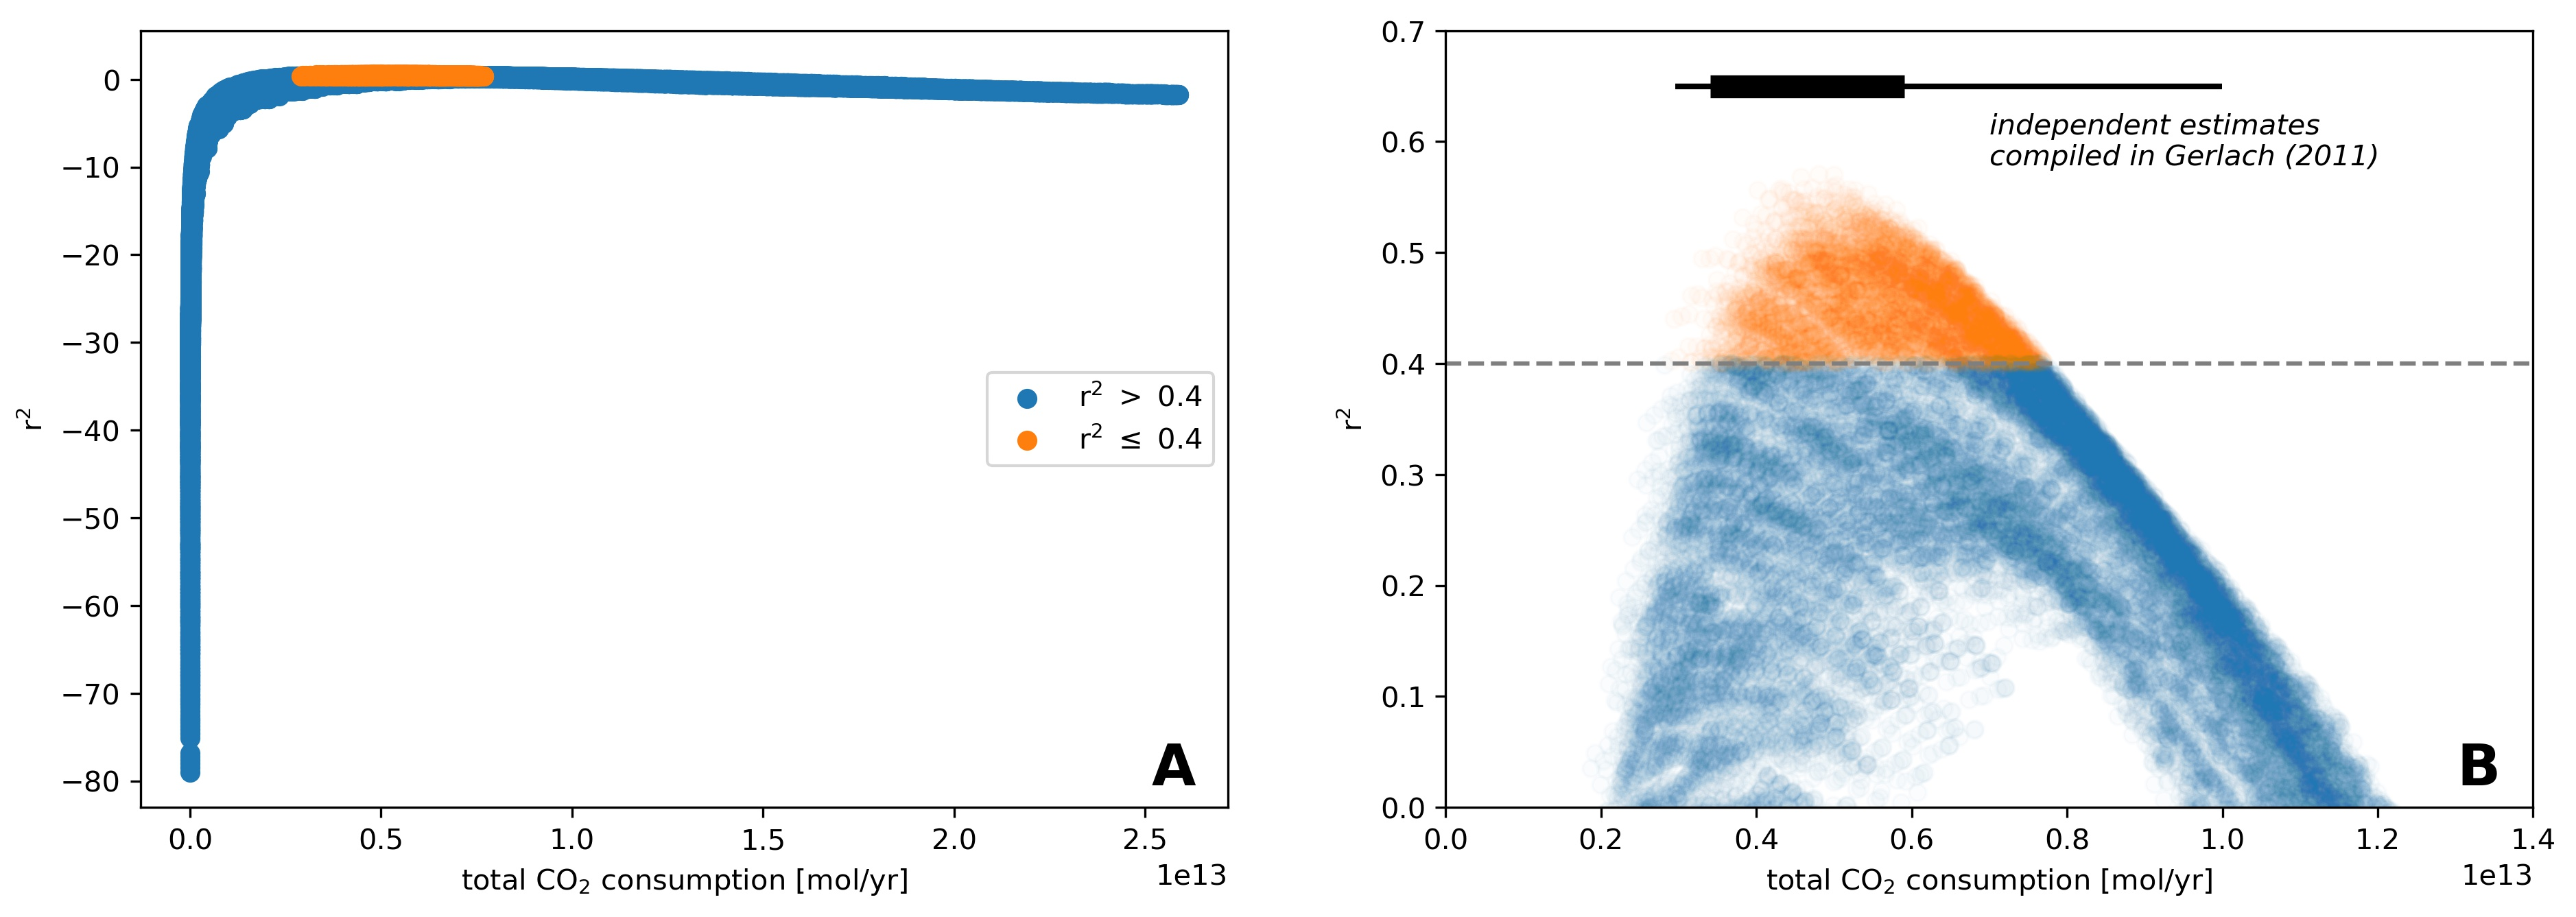
\includegraphics[width=1\textwidth]{Manuscript/Figures/W_vs_r2.jpg}
    \caption{\textbf{A)} Modeled global \COtwo consumption vs. the coefficient of determination ($r^{2}$) between modeled and data-constrained \COtwo consumption in each of the watersheds. Each point represents model output using one of the 78,000 parameter combinations. \textbf{B)} Same as A, but zoomed to the plotting space with positive $r^{2}$'s. The black line represents the full range of estimates of the present-day global CO$_{2}$ emission rate compiled in \citet{Gerlach2011a}. The black box represents the preferred range of those estimates.}
    \label{fig:W_vs_r2}
\end{figure}

\begin{figure}[h!]
    \centering
    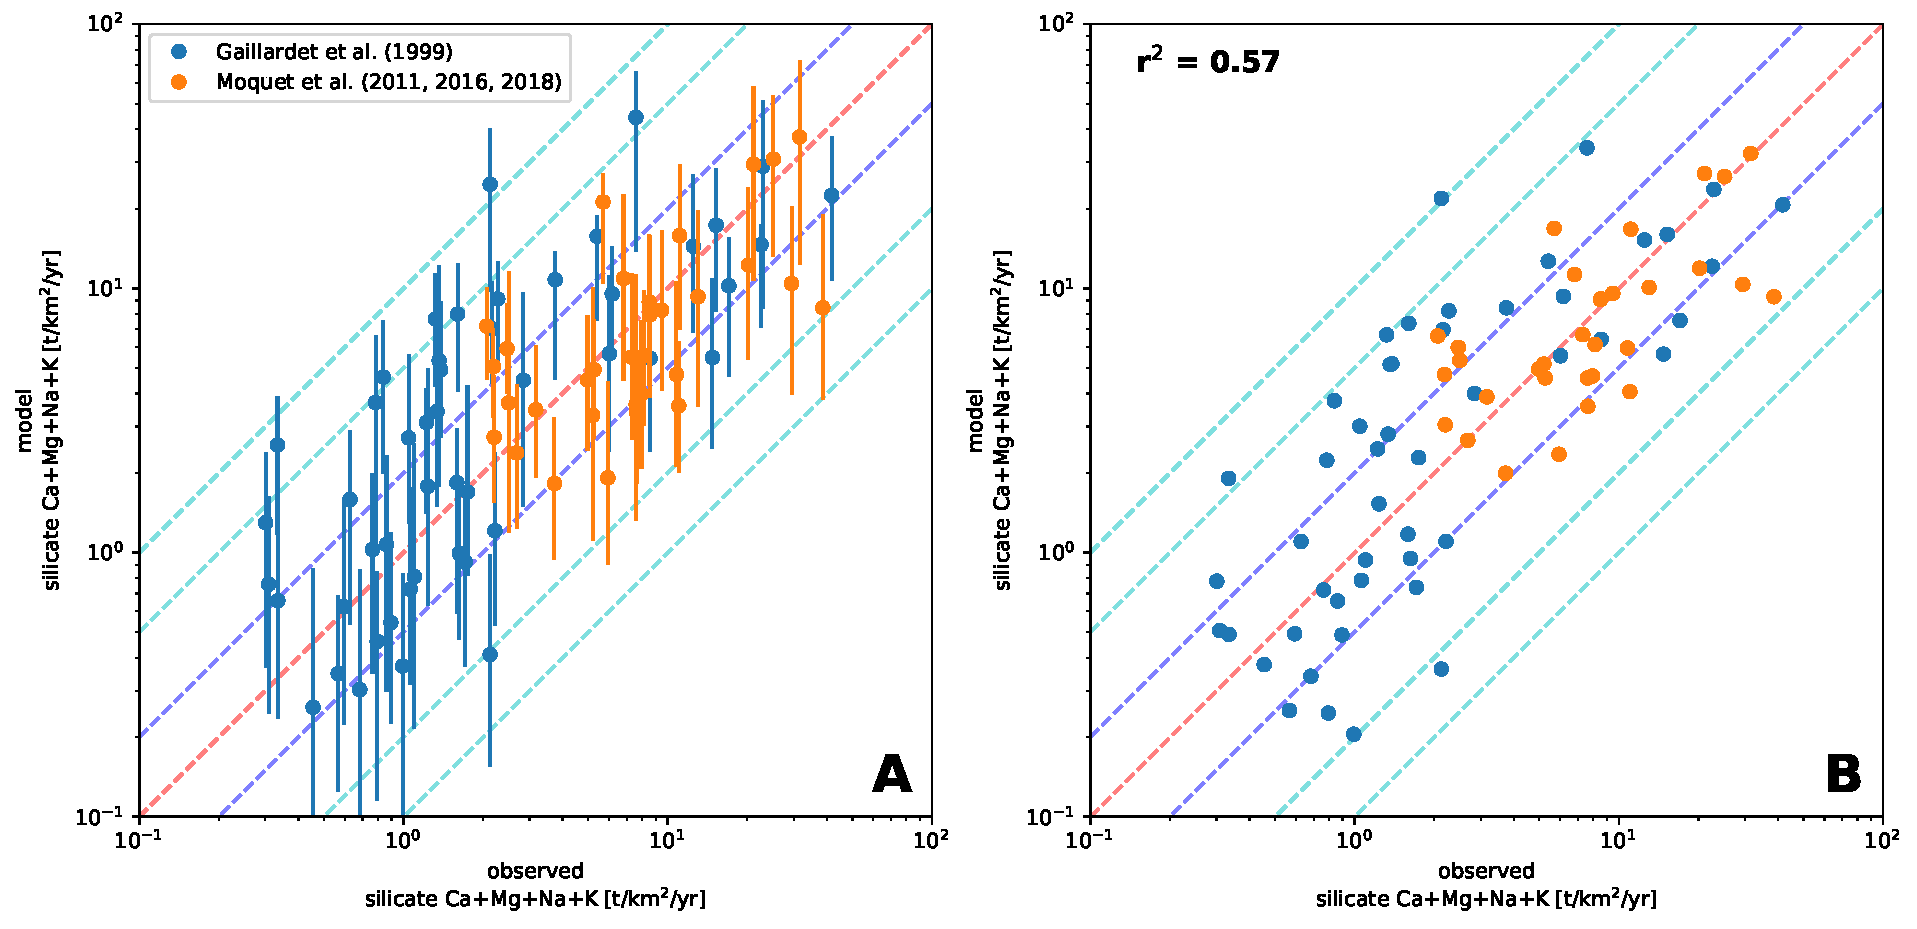
\includegraphics[width=1\textwidth]{Manuscript/Figures/r2_cross_plot.pdf}
    \caption{Modeled vs. data-constrained \COtwo consumption in watersheds around the world. \textbf{A)} Each point represents a single watershed, and the y-value of the point shows the mean value of the 3,339 parameter combinations that produce individual watershed \COtwo consumption fluxes that approximate those estimated in the literature for the present-day. Whiskers extend to the minimum and maximum modeled watershed \COtwo consumption fluxes for the 3,339 parameters combinations. The red dashed line is the 1:1 line, the blue dashed line is the 2:1 line, and the cyan dashed lines are the 5:1 and 10:1 lines. \textbf{B)} Same as A, but only showing the parameter combination that produced that highest $r^{2}$.}
    \label{fig:r2_cross_plot}
\end{figure}

The majority of the original 78,000 parameter combinations produce \COtwo consumption maps with poor fits to the measured watershed data (Fig. \ref{fig:W_vs_r2}). Given that the coefficient of determination ($r^{2}$) is calculated using equation \ref{eq:10} rather than fitting a linear model, many of the combinations associated with particularly poor fits result in negative $r^{2}$ values (Fig. \ref{fig:W_vs_r2}). However, given the right permutation of parameters, GEOCLIM produces \COtwo consumption maps that fit the measured watershed data reasonably well. We therefore eliminate all parameter combinations that produce a $r^{2}<0.4$, which leaves 3,339 unique parameter combinations (Figs. \ref{fig:W_vs_r2} and \ref{fig:r2_cross_plot}).

Global CO$_{2}$ consumption calculated from these 3,339 parameter combinations ranges from 2.7$\times10^{12}$~mol/yr to 7.1$\times10^{12}$~mol/yr, with a mean of 5.4$\times10^{12}$~mol/yr. These estimates fall within the range of those independently estimated in the literature for the present-day: the full range of estimates of the present-day global CO$_{2}$ emission rate compiled in \citet{Gerlach2011a} is 3.0--10.0$\times10^{12}$~mol/yr, with the preferred range of those estimates being 3.4--5.9$\times10^{12}$~mol/yr (Fig. \ref{fig:W_vs_r2}B).

\section*{Climate Model}

We use temperature and runoff fields from a subset of the GFDL CM2.0 experiments (\citealp{Delworth2006a, Delworth2006b}; available for download at \url{https://nomads.gfdl.noaa.gov/dods-data/gfdl_cm2_0/}) for the climate model component of GEOCLIM. These experiments were performed in order to explore the effect of various changes in forcing agents on climate since ca. 1860 at a 2.0\degrees $\times$ 2.5\degrees resolution. In the ``1860 control'' experiment, forcing agents representative of conditions ca. 1860 (including \COtwo, CH$_{4}$, N$_{2}$O, O$_{3}$, sulfates, carbon, dust, sea salt, solar irradiance, and the distribution of land cover types) are held constant for 500 years after reaching equilibrium. \pCOtwo in 1860 is assumed to be 286~ppm. In the ``+1\%/yr to 2$\times$'' experiment, initial conditions are taken from the ``1860 control'' experiment, then \pCOtwo is prescribed to increase from 286~ppm at a compounded rate of +1\% per year for 70 years, when \pCOtwo reaches double (572~ppm) of the initial value. \pCOtwo is then held constant until the end of the 280 year experiment. All non-\COtwo forcing agents are held constant. The ``+1\%/yr to 4$\times$'' experiment is identical to the ``+1\%/yr to 2$\times$'' experiment, except that \pCOtwo is prescribed to increase for 140 years, when \pCOtwo reaches quadruple (1144~ppm) of the initial value. \pCOtwo is then held constant for 160 years. We take the mean of the last 100 years of each of these three experiments (when \pCOtwo is being held constant at its final level) to obtain temperature and runoff fields for 286, 572, and 1144~ppm respectively. Temperature and runoff fields for any arbitrary \pCOtwo value between 286 and 1144~ppm is obtained by interpolating between the three modeled \pCOtwo levels.

\section*{Indonesia and New Guinea Scenarios}

\begin{figure}[h!]
    \centering
    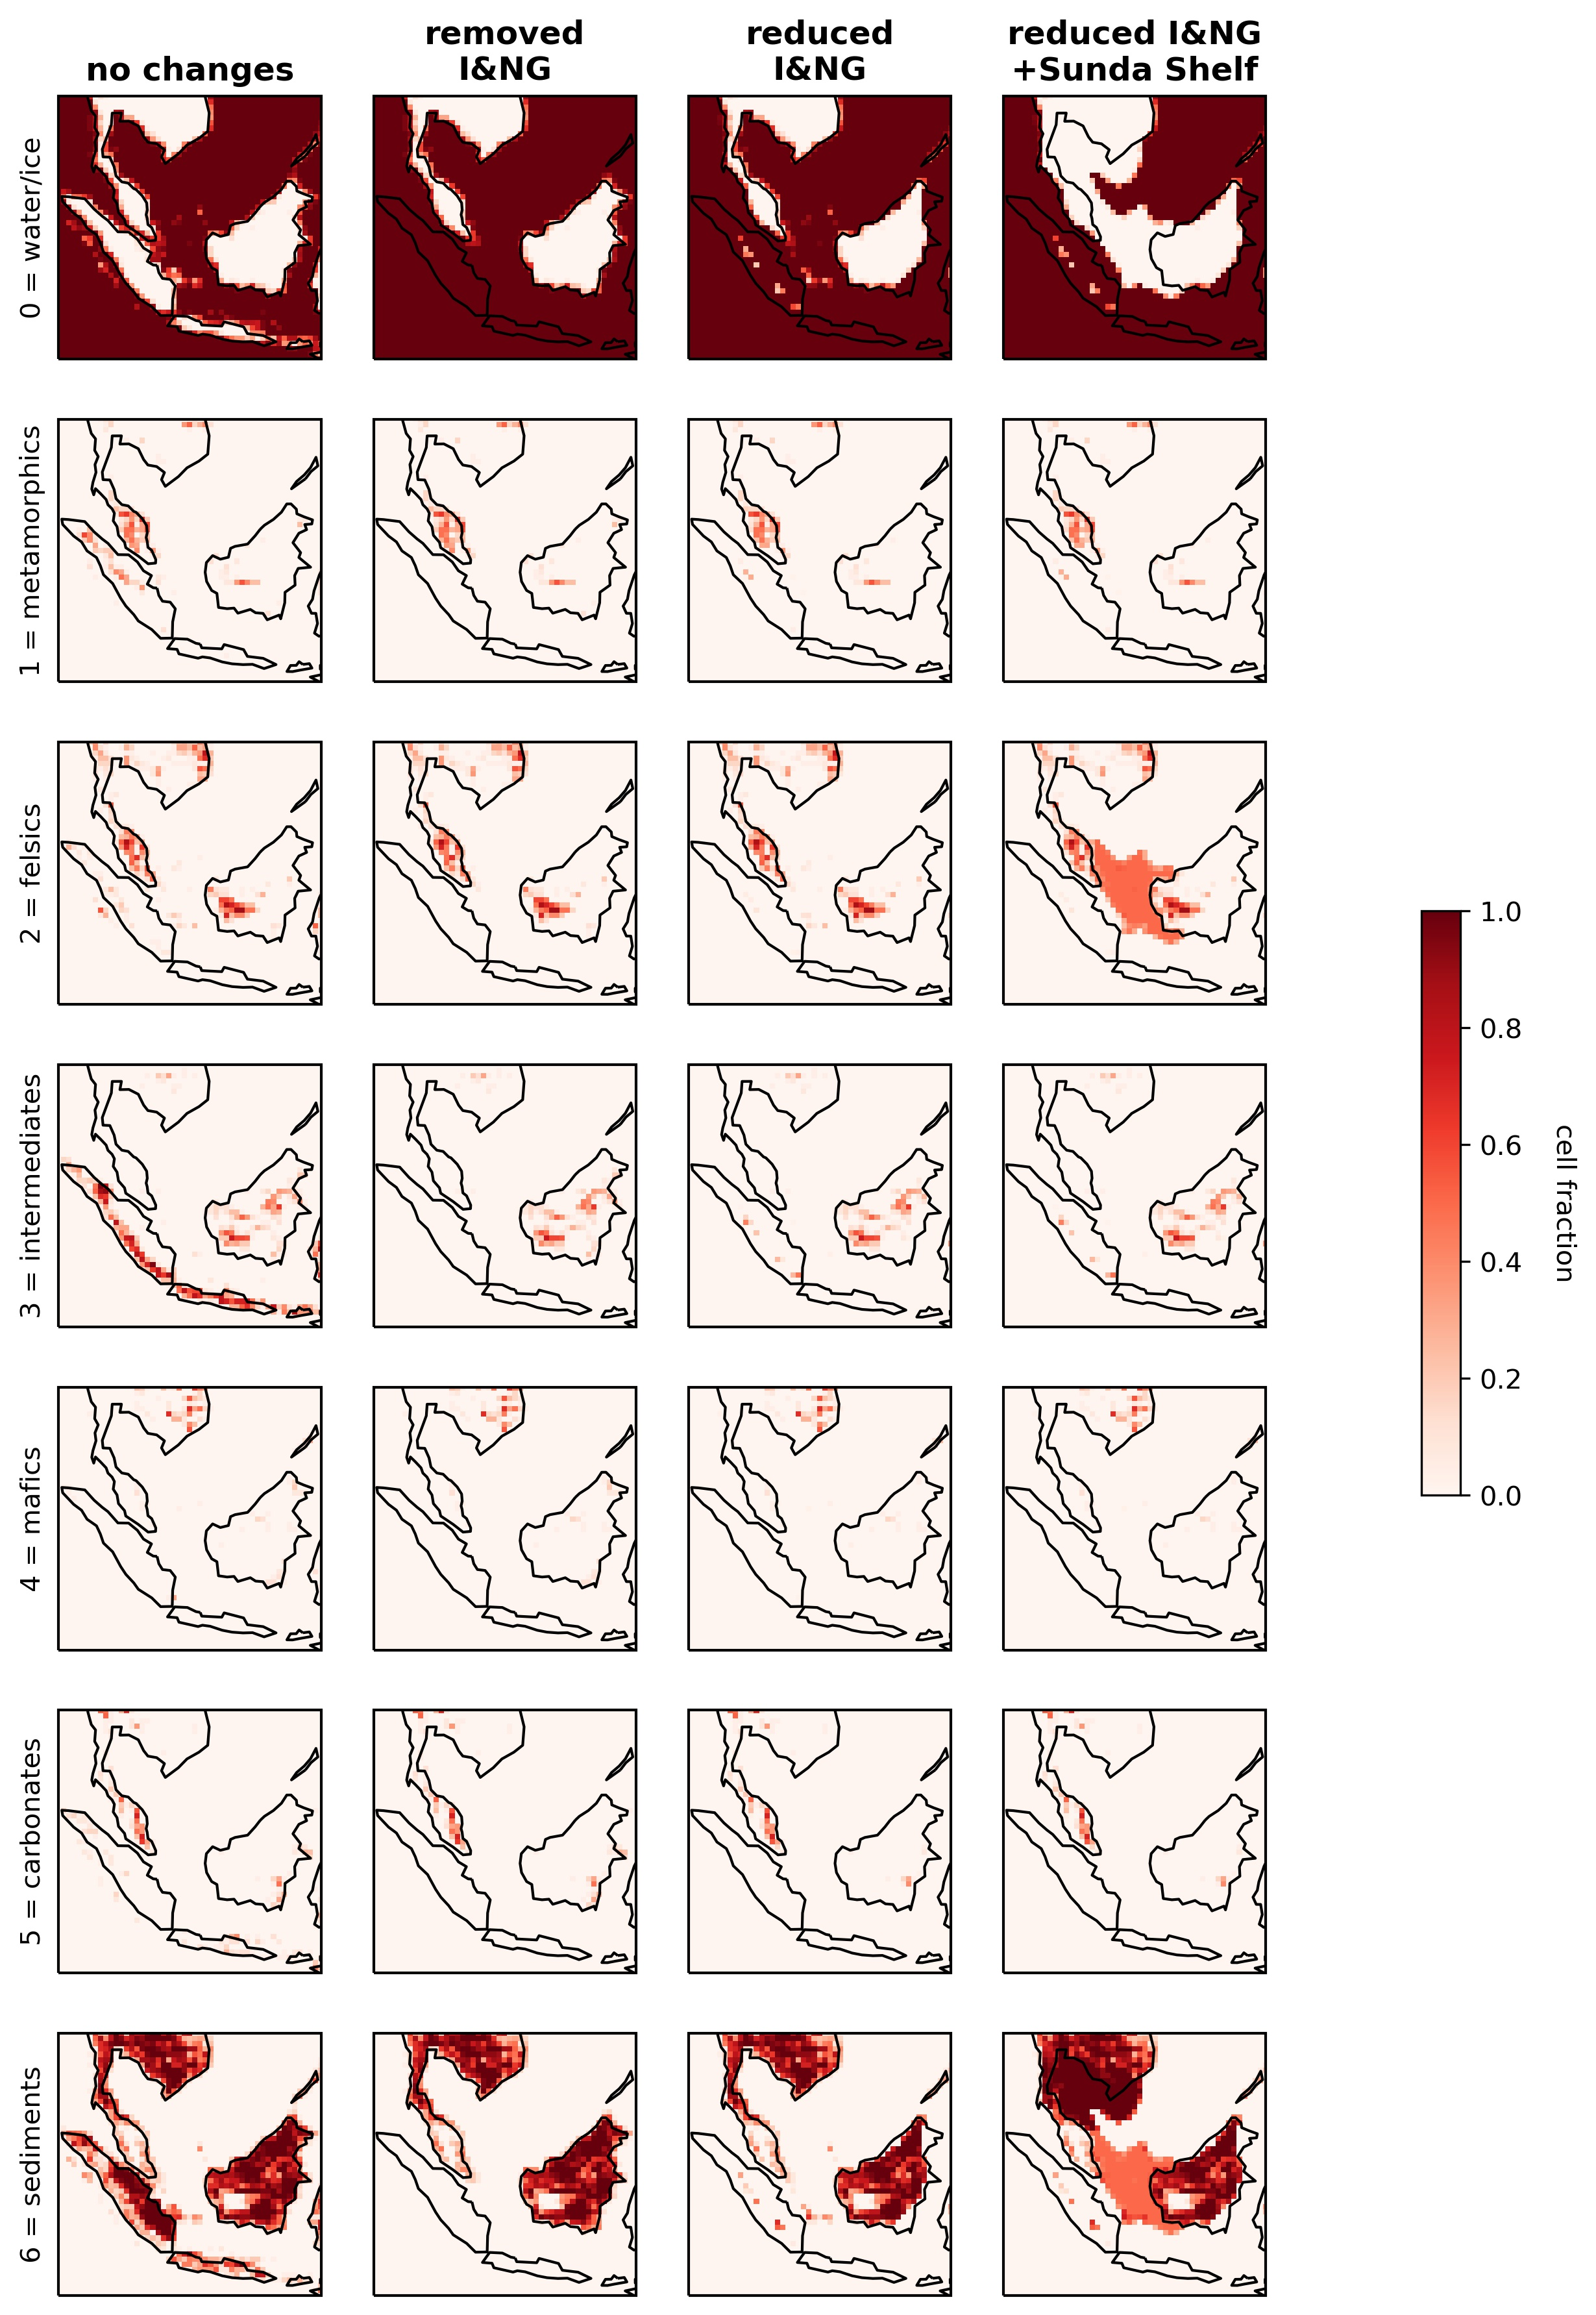
\includegraphics[width=1\textwidth]{Manuscript/Figures/ING_fracs.jpg}
    \caption{0.5\degrees $\times$ 0.5\degrees lithologic maps of Indonesia and New Guinea (I\&NG) used to force GEOCLIM. Only the 15~Ma scenarios are shown here, but the 10 and 5~Ma scenarios would be similar, using the 10 and 5~Ma shorelines shown in Figure 1 of the main text instead. Each column represents a tested scenario. Each row represents a lithologic category. Solid black lines show present-day shorelines.}
    \label{fig:ING_fracs}
\end{figure}

\begin{figure}[h!]
    \centering
    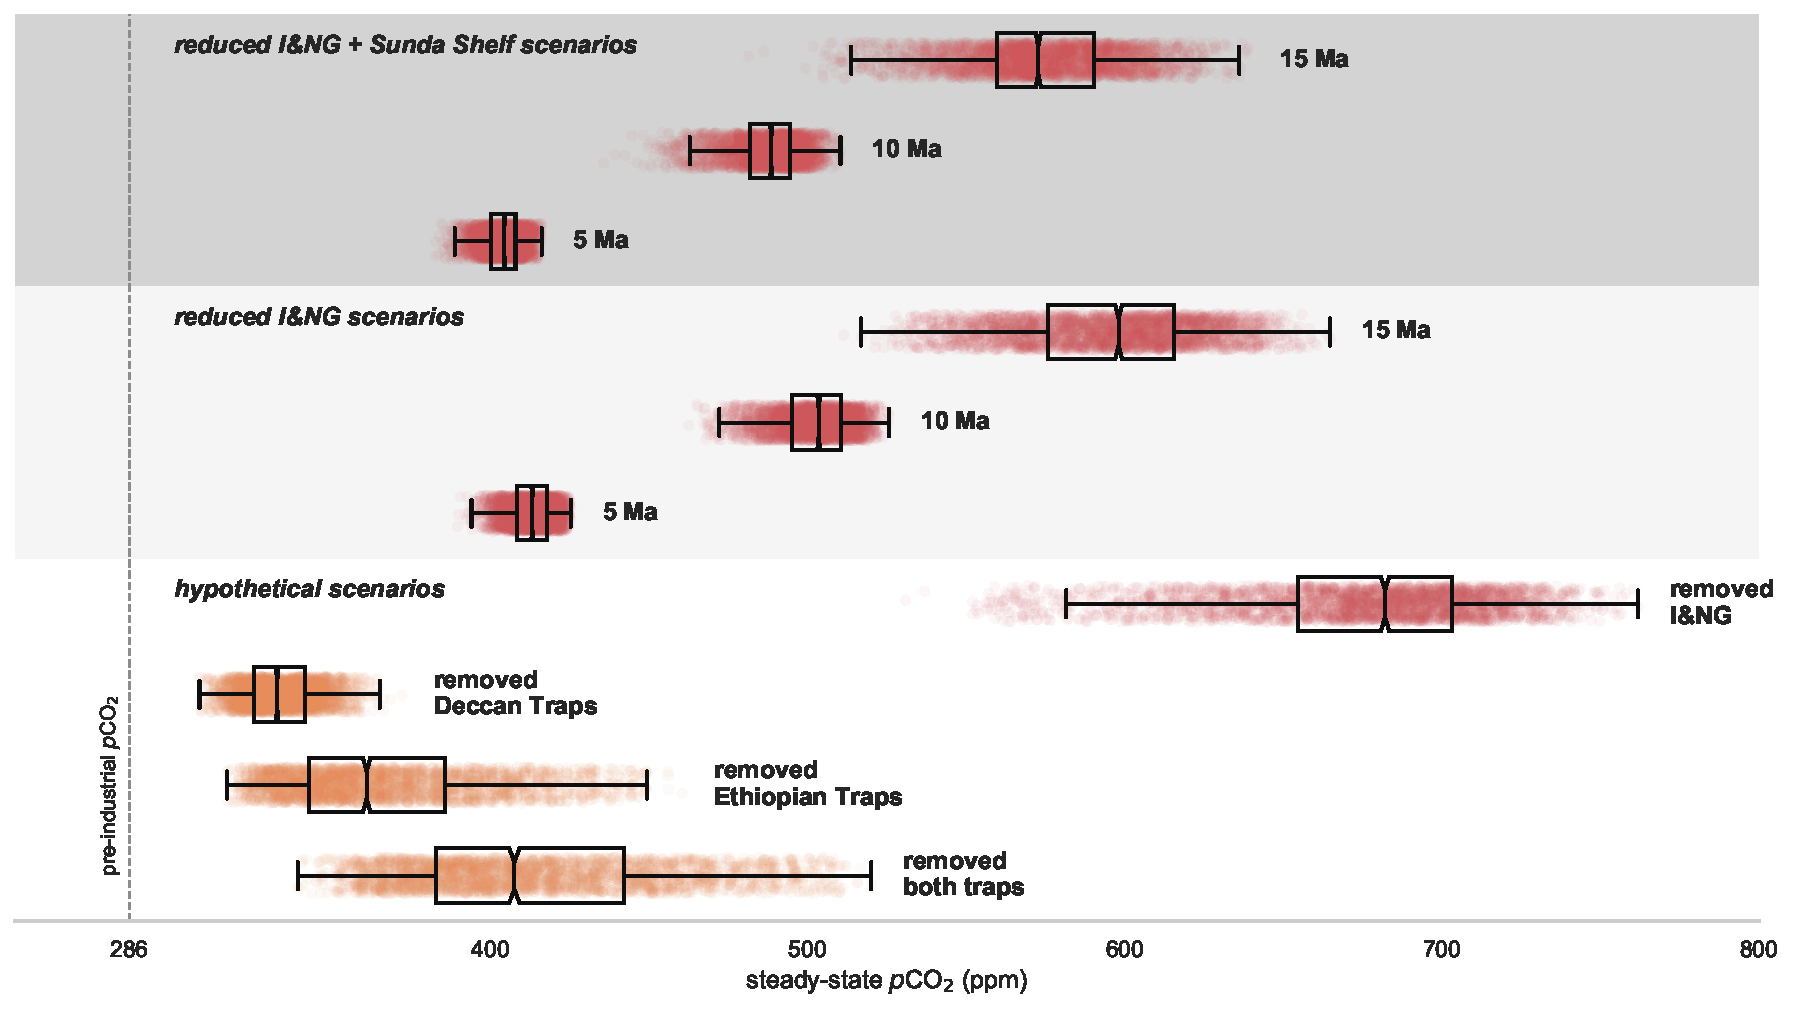
\includegraphics[width=1\textwidth]{Manuscript/Figures/scenario_pCO2_all.pdf}
    \caption{Steady-state \pCOtwo estimates from GEOCLIM for the various scenarios discussed in the text. For each of the ten scenarios, each point represents an estimate from one of the 3,339 unique parameter combinations that resulted in reasonable total global \COtwo consumption and most closely matched \COtwo consumption estimated from watershed data (see SI). The box encloses the middle 50\% of the \pCOtwo estimates (i.e. the interquartile range), and the notch represents the median with its 95\% confidence interval. The whiskers extend to 1.5$\times$ the interquartile range, or to the minimum/maximum of the estimates if no estimates are below/above this range.}
    \label{fig:scenario_pCO2_all}
\end{figure}

We use geological data to quantify the changes in the area of I\&NG over the past 20~m.y (described in detail in \textit{Paleoshoreline Reconstruction and Geological Synthesis}). To generate the lithologic map used in the ``removed I\&NG'' scenario (Fig. \ref{fig:ING_fracs}), we remove all land associated with arc-continent collision in I\&NG. To generate the lithologic map used in the ``reduced I\&NG + Sunda Shelf'' scenarios (Fig. \ref{fig:ING_fracs}), we take the estimated paleoshorelines of I\&NG for 15, 10, and 5~Ma, then remove all land that falls outside of these bounds. The slope and lithologic classification of each pixel is identical to that of the present day, provided that these pixels fall within the estimated paleoshorelines of I\&NG for their respective time slice. We then add land that is not exposed today (i.e. the Sunda Shelf). However, the assignment of lithology, runoff, and slope for pixels on the Sunda Shelf is not trivial, given that the shelf is not currently exposed. As discussed in \textit{Paleoshoreline Reconstruction and Geological Synthesis}, the Sunda Shelf is a flat-lying, relatively stable platform of continental crust. Basement highs between Malaysia/Sumatra and Borneo are typically granitic and bounded by basins dominated by shallow marine clastic fill. However, basement highs are less common in the Gulf of Thailand. We therefore assign all pixels of the Sunda Shelf to be 50\% felsic and 50\% sediment, except in the Gulf of Thailand where pixels are assigned to be 100\% sediment. For the slope, we take the mean slope value (0.0038~m/m) of relatively flat land on eastern Sumatra, and assign this value to all pixels of the Sunda Shelf.  For the runoff, we linearly interpolate along latitude bands between present-day land pixels to obtain runoff values for the presently-submerged Sunda Shelf. This approach preserves large N-S variation in runoff associated with the large-scale Hadley circulation and therefore should be reasonable to first-order, although it does not accurately capture the smaller-scale interactions between land and ocean/atmosphere circulation.

To explore the sensitivity of our results to the inclusion of the Sunda Shelf, we also tested ``reduced I\&NG'' scenarios for 15, 10, and 5~Ma, which are identical to that of the ``reduced I\&NG + Sunda Shelf'' scenarios without the addition of the Sunda Shelf. We find that the estimated steady state \pCOtwo's for the ``reduced I\&NG'' scenarios are only marginally higher than those of the ``reduced I\&NG + Sunda Shelf'' scenarios (Fig. \ref{fig:scenario_pCO2_all}), suggesting that our results are largely insensitive to the inclusion of the Sunda Shelf. This insensitivity can be attributed to the low Ca+Mg concentrations of felsic and sediment lithologies in conjunction with the low slope values distributed across the shelf.

The decrease in \pCOtwo that we estimate associated with the emergence of I\&NG since 5~Ma ($\sim$120~ppm) is greater than that proposed in \citet{Molnar2015a} ($\sim$19~ppm). This 19~ppm value in \citet{Molnar2015a} is obtained from an equation that assumes a direct linear relationship between mean global temperature and changes in weathering-rate-weighted land area, scaled by a factor $\alpha$ that is intended to account for the influence of both runoff and temperature (Equation 3 in \citealp{Molnar2015a}). \pCOtwo is then estimated from $T$ using a simple energy balance equation. However, as discussed in the main text, as \COtwo sinks are removed and \pCOtwo rises, temperature increases and the hydrological cycle is invigorated, causing other weathering sinks to increase until a new steady-state is achieved at higher \pCOtwo. The linear relationship described in Equation \ref{eq:Molnar3} ignores these feedbacks in the global climate system.

\section*{Limitations and Future Directions}

As with any modeling study, there are limitations with the approach. We consider one of the current limitations to be the climate model component of GEOCLIM that was used in this study (GFDL CM2.0) has a lower spatial resolution (2.0\degrees $\times$ 2.5\degrees) than what can be achieved with the latest climate models and computational resources. While this model is effective in capturing the large-scale climatology, using an updated climate model at higher resolution may result in runoff and temperature fields with different spatial distribution and sensitivities to elevation.

Another limitation associated with using a modern-day climate model, is that in the scenarios with varying shorelines, we hold the slope and lithology to be the same as the present-day in each pixel. This means that while we are changing the amount of emergent land, we are not changing the latitudinal or longitudinal position and are keeping the slope of any emerged pixel the same. Given that similar distributions of lithology and slope are reasonable in the past and that latitudinal translation has been relatively minor (Fig. XXX), we consider this simplification to be reasonable to first-order. However, implementing high-resolution climate models with both varying shorelines and changes in paleogeographic position for these scenarios is a valuable future direction. Additionally, such modeling efforts could give insight into whether associated changes in ocean and atmosphere circulation would have significantly modulated precipitation in I\&NG.  Given that precipitation in this region is primarily driven by large-scale convective upwelling leading to high precipitation over both land and water, the current approach is a reasonable approximation for I\&NG. However, for paleogeographic change that would have very significantly modified precipitation over broad swathes of land such as growth of the Himalaya, this approach of using modern climate model results is not viable.

Finally, although the silicate weathering component of GEOCLIM now implements lithology-dependent Ca+Mg concentration, our implementation does not include lithology-dependent kinetics of mineral dissolution. Relative to felsic lithologies, mafic lithologies contain a higher concentration of minerals with faster dissolution kinetics (e.g. plagioclase). However, Ca+Mg from both felsic and mafic lithologies is predominantly sourced from minerals with faster dissolution kinetics, and we therefore use the same chemical weathering formulation (including the same activation energy) across lithologies. We also do not include the effects of reverse weathering \citep{Michalopoulos1995a} as it is not clear how it should be parameterized and it is interpreted to be relatively minor flux in the Cenozoic \citep{Isson2018a}. Formation of authigenic clays that scales with Ca and Mg concentration of riverine waters could decrease the \COtwo consumption associated with silicate weathering although the overall trend seen in this study would remain.

\section*{Paleoshoreline Reconstruction and Geological Synthesis}

Geological maps, stratigraphic data, and previous paleoshoreline compilations were used to calculate the changes in different types of subaerially exposed rocks in I\&NG. Following \citet{Molnar2015a}, we analyzed the area changes of islands that are larger than $\sim$200~km$^{2}$ (Fig. 1 in main text). We also included changes in areas of submerged continental shelves that were previously exposed, like the Sunda Shelf. Larger islands were further divided into regions based upon their position on microplates as defined by \citep{Matthews2016a}. Miocene to present stratigraphic columns were compiled from each region to develop an age model for paleoenvironmental indicators. In general, carbonate strata and thin-bedded siliciclastic strata were assumed to be deposited in a subaqueous marine environment, whereas evidence for exposure and terrestrial siliciclastic deposits were used as indicators of a subaerial paleoenvironment. Following previous paleoshoreline compilations and these environmental indicators, paleoshorelines were outlined in QGIS to calculate areas for the Early Pliocene (5 Ma), Late Miocene (10 Ma), and Middle Miocene (15 Ma). The paleoshoreline reconstructions within the paleogeographic models broadly coincide with sub-Epoch boundaries (i.e. Early Miocene = 23--16~Ma, Middle Miocene = 15.99--11.61~Ma, Late Miocene = 11.6--5.4~Ma, Pliocene =5.39--3.8 Ma) but we recognize that the biostratigraphic resolution is an additional source of uncertainty.

Several new sources for paleoshoreline data have become available since \citet{Molnar2015a}. Particularly, for Sulawesi, we followed the recent stratigraphic compilation and paleoshorelines delineated by \citet{Nugraha2018a}, and in New Guinea, we followed \citet{Gold2017a} and \cite{Harrington2017a}. Although the outlines of our paleoshorelines are significantly different from those used for 5~Ma by \citet{Molnar2015a} our calculated area is comparable. 

\subsection*{Malay Peninsula and Sunda Shelf}

Paleogeographic reconstructions of Peninsular Malaysia suggest that it has been largely exposed over the last 20~Ma \citep{Hall2002a, Hall2013b}. Although the majority of the Sunda Shelf is currently submerged, large portions of this flat-lying, relatively stable platform of continental crust were also emergent throughout the Neogene, and were repeatedly subaerially exposed during the Pleistocene as recently as the Last Glacial Maximum \citep{Hall2002a}. Similarities between the terrestrial biotas of Borneo and mainland Southeast Asia confirm the existence of land bridges on the Sunda Shelf throughout the Miocene \citep{Moss1998a}. Eocene through Miocene rifting of the South China Sea resulted in subsidence throughout the Sunda Shelf \citep{Morley2013a}. Grabens associated with this subsidence became freshwater rift lakes that later transitioned to partially enclosed inland seas and extensive brackish or saline wetland environments. Palynological analysis suggests widespread swamp environments persisting through the Late Miocene \citep{Morley2013a}. Basement highs (e.g. the Natuna Arch, currently subaerially exposed as the largely granitic island of Natuna off SW Borneo, as well as the granitic Tin Islands south of the Malay Peninsula) are typically bounded by Paleogene to Neogene basins dominated by shallow marine clastic fill \citep{Darmadi2007a}. Most paleogeographic reconstructions of the region incorporate some degree of exposure of the Sunda Shelf from 20~Ma onwards \citep{Hall2013b, Madon2013a}, although it is omitted in the 5~Ma paleogeographic model of \citet{Molnar2015a}.

\subsection*{Borneo and Palawan}

Our reconstructions of the paleoshorelines of Borneo and Palawan are largely informed by extant paleogeographic constructions detailed in \citet{Hall2001a, Hall2013a, Hall2013b},  as well as geologic maps and local shoreline reconstructions found in \citet{vandeWeerd1992a, Witts2012a, Madon2013a, Kessler2015a}. Comprised of Paleozoic to Mesozoic crustal components that were largely accreted to Sundaland by the late Cretaceous \citep{Metcalfe2013a}, the southern and western portions of Borneo (SW Kalimantan) have been subaerially exposed throughout the Neogene \citep{Hall2013a, Hall2013b}. A collision along the northern margin of Borneo associated with the initiation of rifting in the South China Sea resulted in the late Eocene uplift of the Central Range mountains \citep{Hutchison1996a}, which provide sediment to basins along the Southern (Kalimantan) and northern (Sabah and Sarawak) coasts of the island. In the east, the Barito, Kutei, and Tarakan basins developed as a single area of subsidence (associated with the opening of the Makassar Straits in the Eocene) before the basins were isolated by Oligocene faulting and Miocene uplift \citep{Witts2012a}. The Kutei Basin is characterized by eastward-prograding deltaic and shallow shelf deposits that have been steadily supplied with sediment from the Schwaner Mountains of SW Kalimantan and the Central Range \citep{vandeWeerd1992a}. North of the Kutei Basin, the deltaic deposits found in the Tarakan Basin similarly prograde eastward from the mid Miocene onward, fed by the northern drainages of the Central Range \citep{Satyana1999a}. In SE Kalimantan, the Barito Basin is bounded to the east by the ophiolite-bearing Meratus Mountains. Sedimentological data suggests that the Meratus Mountains were not emergent until the Late Miocene \citep{Witts2012a}.

Separated from the Paleozoic continental core of SW Borneo by the Lupar Line suture zone, the northern portion of Borneo (Sabah) is underlain by ophiolitic basement that extends to Palawan \citep{Hall2008a, Ilao2018a}. The Sarawak Basin and NW Borneo trough offshore Sabah host $>$10~km-thick Neogene sedimentary sequences, indicative of the extent and duration of exhumation in northern Borneo \citep{Hall2008a}. The Late Oligocene/Early Miocene Sabah Orogeny resulted in the uplift of both Sabah and southern Palawan \citep{Hall2013a}, as well as the obduction of the Palawan ophiolite and Telupid ophiolite of northern Sabah. Under-thrusting of thinned passive-margin continental crust beneath these suprasubduction ophiolites resulted in Early to Middle Miocene exhumation and offshore unconformities \citep{Hall2008a}. Early Miocene sediments in northern Sabah have a provenance from Palawan \citep{Suggate2014a}, indicating that Palawan, like northern Borneo, experienced uplift during the Sabah orogeny. However, initiation of back-arc extension in the Sulu Sea around 19~Ma \citep{Hall2013a} resulted in the subsidence of the eastern Palawan Mountains, eliminating or reducing the role of Palawan as a sediment source for the Borneo trough. The 14~Ma Capoas Granite on Palawan and the 7.5~Ma Kinabalu Granite in Sabah are interpreted to be the result of crustal thinning related to pulses of regional backarc extension \citep{Hall2013a}. Thermochronological data from the Sabah highlands suggest extremely rapid uplift (7~km/m.y.) and exhumation during the latest Miocene and early Pliocene, resulting in the recent formation of Mt. Kinabalu, the tallest peak in Borneo \citep{Cottam2013a}.

\subsection*{Sulawesi}

For the paleoshorelines of Sulawesi, we largely followed the recent stratigraphic compilation and paleoshorelines compilation of \citet{Nugraha2018a}. Geographically, Sulawesi can be divided into a central highland region flanked by North, South, Southeast, and East Arms. These arms have high relief ($>$3~km) that are separated by deep basins and broadly define Sulawesi's seven tectonic provinces: 1) the West Sulawesi magmatic arc of the South Arm, 2) the Central Sulawesi metamorphic Belt, 3) the Sangihe arc of the North Arm, 4) the East Sulawesi Ophiolite of the East Arm, 5) the southeast metamorphic belt of the Southeast Arm, and the microcontinental blocks of 6) Banggai-Sula and 7) Buton-Tukang Besi \citep{Hamilton1979a, Katili1978a}. Like SW Borneo, the North and South Arms and much of Central Sulawesi are underlain by continental blocks that rifted off of the Australian-Birds Head margin in the Jurassic and collided in the Cretaceous with Eurasian basement of Sundaland as part of the Woyla Arc system \citep{Parkinson1998b, Hennig2016a, Hall2017a, Hennig2017a}. After collision, subduction polarity reversed and a Cretaceous to Miocene SE-facing volcanic arc developed \citep{Polve1997a, Elburg1998a} that was connected to the paleo-Sunda Arc \citep{Hall2002b}, also referred to as the Great Indonesian arc \citep{Harris2006a}.  The ophiolites of Sulawesi were generated in this arc system in a back arc to intra-arc setting (\citealp{Monnier1995a}, but see \citealp{Kadarusman2004a} for an alternative view), and the largest fragments of the East Sulawesi ophiolite were detached from their metamorphic sole in the late Oligocene (32--28~Ma; \citealp{Parkinson1998a}) and thrust to the east above a west dipping slab (East Sulawesi block of \citealp{Villeneuve2001a}). During the Early to Middle Miocene, the Tukang Besi-Buton block began to collide obliquely with the southeastern end of the Sunda Arc, causing ophiolite emplacement in West and SE Sulawesi, including Buton \citep{Smith1991a, Bergman1996a}. 

The North Arm consists of Late Pliocene and younger volcanic rocks built upon Eocene to Early Miocene oceanic basalt, basaltic andesite, pelagic sediments, and metamorphic rocks \citep{Elburg1998a}. Eocene to Early Miocene volcanic rocks formed above a NW dipping slab in an arc system that extended to West and South Sulawesi \citep{vanLeeuwen2005a}. Gorontalo Bay is an extensional basin that formed in the Pliocene, and prior to that time, the East Sulawesi was attached to the North Arm of Sulawesi. After the Oligocene to Early Miocene accretion of the East Sulawesi ophiolite, the arc system stepped out to the SE forming a Neogene (23--16~Ma) volcanic belt on the East arm \citep{Kadarusman2004a}. In the Late Miocene, SE-dipping subduction was initiated below the North Arm, which continues today at the North Sulawesi Trough. North Sulawesi was not substantially emergent until the Pliocene \citep{vanLeeuwen2005a}. Active volcanoes extend from the North Arm through the Sangihe Arc into the southern Philippines. 

The East and Southeast Arms consist predominantly of mafic and ultramafic rock of the East Sulawesi Ophoilite that is exposed for more than 10,000~km$^{2}$ \citep{Monnier1995a}. The East Arm preserves a complete ophiolitic sequence underlain by a metamorphic sole, m\'elange, imbricate continental margin and crystalline basement with a blueschist metamorphic overprint \citep{Silver1983a, Monnier1995a, Parkinson1998a}. Locally, the structural thickness of the ophiolite exceeds 15~km with surface relief over 3~km \citep{Kadarusman2004a}. Seventeen igneous K-Ar dates from the East Sulawesi ophiolite range from 93--32~Ma, clustering between 60~Ma and 40~Ma (\citealp{Parkinson1998b} and references therein). K-Ar dates on hornblende from the metamorphic sole yielded cooling ages between 36--23~Ma \citep{Parkinson1998a, Villeneuve2001a}, which dates the initial emplacement of the East Sulawesi ophiolite as the north Sulawesi volcanic arc was underthrusted by the Sula spur (Australian crust) \citep{Silver1983a, Parkinson1998a}; however, despite these relatively old ages of emplacement, it appears that the ophiolites on the East Arm were not substantially subaerially exposed and exhumed until the Miocene.  

Collision of the Sula-Banggai block with the East margin of Sulawesi began in the latest Miocene and uplift accelerated in the early Pliocene (5.2~Ma to 3.8~Ma) and is associated with a major pulse of sedimentation in adjacent basins \citep{Davies1990a, Villeneuve2000a}. Off the northeast margin of the east arm of Sulawesi, Miocene platform carbonates on the Sula-Banggai block are overlain by Late Miocene to Early Pliocene ophiolite detritus in the Celebes m\'elange \citep{Davies1990a}. Thus, although the East Sulawesi ophiolite was trapped/emplaced onto the composite Sundaland margin (i.e. a fragment of previously accreted Australian crust) between 36~Ma and 23~Ma, mafic and ultramafic rocks on the south and west arms appear to have not been substantially subaerially exposed in the south and west arms until after 15~Ma, and on the east arm until after 5~Ma.

West Sulawesi rifted from Borneo during the Eocene forming the Makassar Straits back arc basin behind a southwest-facing arc \citep{Polve1997a}. Eroded fragments of ophiolite and extensive belts of volcanic rocks are preserved on the West and South Arms of Sulawesi \citep{Bergman1996a, vanLeeuwen2010a}. During the Middle Miocene (ca. 15--13~Ma), extensional faults in the Bone basin reversed, which was accompanied by uplift and erosion of the Bone Mountain ophiolite and Lamasi complex in West Sulawesi \citep{Bergman1996a, vanLeeuwen2010a}. Shortening was likely due to the collision of the leading edge of the Buton-Tukang Besi block, which collided with Buton and the SE Arm of Sulawesi \citep{Smith1991a}. Uplift and erosion is recorded by the presence of a major Middle Miocene unconformity and sedimentary breccias in marginal basins \citep{Bergman1996a, vanLeeuwen2010a}. Uplift was diachronous, not effecting units below and to the west of the Lamasai ophiolite until the Middle Miocene (ca. 13~Ma) \citep{vanLeeuwen2010a}. Alkali volcanism ensued at ca. 11~Ma and is associated with a second phase of extension and exhumation. From the Late Miocene to Pliocene fission track ages imply deep exhumation \citep{Smith1991a, Bergman1996a, vanLeeuwen2010a}.

Fission track ages from granitoids in central Sulawesi indicate rapid uplift of Central Sulawesi (200--700~m/m.y.) starting at about 5~Ma associated with movement on the Palo-Koro fault \citep{Bellier2006a}. The fault system also shows a normal component with rapid exhumation of rock west of the fault in western Sulawesi -- all fission track dates are younger than 5~Ma \citep{Bellier2006a}. Just east of the Palo-Koro fault, the Palu Metamorphic Complex was exhumed in the Late Miocene to early Pliocene in the north (ca. 5.3~Ma) and later Pliocene in the south (ca. 3.1--2.7~Ma) at rates of up to 400~m/m.y. \citep{Hennig2017b}.

\subsection*{New Guinea and Halmahera}

Paleoshoreline maps were georeferenced from several previous tectonic and paleogeographic analyses, most notably those of \citet{Nichols1991a}, \citet{Cloos2005a}, \citet{Gold2017a}, and \citet{Harrington2017a}. These studies were all based to varying degrees on lithological distributions, biostratigraphic, borehole data, and tectonic models. We complimented these data with our stratigraphic compilations for the region to provide further paleoenvironmental context.

Northern New Guinea, including the Melanesian Arc, was emplaced above the Australian plate during the Miocene \citep{Hamilton1979a, Cloos2005a, vanUfford2005a, Baldwin2012a}. Two major ophiolite belts marking the suture -- the Irian-Marum ophiolite belt (including the April ultramafics), and the Papuan Ultramafic Belt (PUB) -- are preserved along the Central Range and Peninsular Range, respectively. South of the Irian-Marum ophiolites, the Ruffaer Metamorphic Complex constructed from the accretionary wedge, forms the spine of the Central Range (up to $\sim$5~km elevation today).

The Middle Miocene (16--14~Ma) basal Makats Formation contains siliciclastic sediment that was transported from the south into the forearc basin associated with the Irian-Marum ophiolite belt \citep{Visser1962a, Cloos2005a}. The beginning of widespread synorogenic sedimentation to the south and on the Australian continental basement was later at ca. 12~Ma \citep{vanUfford2005a}. Mountain building began in Late Miocene time, ca. 8--7~Ma \citep{vanUfford2005a, Baldwin2012a}, but major relief was not generated until the Pliocene \citep{Weiland1996a}. Similarly, the Marum ophiolite was uplifted between 8--5~Ma with 3--4~km of denudation \citep{Crowhurst1996a}. An estimated 80--100~km of shortening has been accommodated by deformation on the south side of the Central Range \citep{Hill1989a, Cloos2005a}.

Along the Papuan Peninsula of Eastern New Guinea, the PUB was obducted above a north dipping slab during Oligocene arc-continent collision between Australian continental fragments and the Melanesian arc, but remained largely subaqueous until the Miocene \citep{Davies1971a, Davies1984a, vanUfford2005a}. Miocene to present arc-continent collision in New Guinea has progressed from west to east. Exhumation of the Central Range accelerated over the past 4~m.y. which is interpreted to be the result of slab-breakoff and buoyant uplift \citep{Cloos2005a}. A change to left-lateral lateral motion on the northern coast of New Guinea at this time, caused the exhumation of ophiolites both along the coast \citep{Monnier1999a} and on the islands Obi \citep{Ali2001a} and Halmahera \citep{Hall1988a, Ballantyne1992a}. In eastern New Guinea, progressive jamming of the north-dipping subduction zone has caused major uplift over the past 4~Ma \citep{vanUfford2005a}, which is well dated with a change in provenance from continental to volcanic detritus \citep{Abbott1994a} and thermochronology \citep{Hill1989a}.

In the Bird’s Neck of western New Guinea, the Lengguru fold belt formed during Middle to Late Miocene clockwise rotation and obduction of the Weyland Terrane \citep{Bailly2009a}. Recent counter-clockwise rotation has exhumed several core complexes and has produced Pliocene compressional deformation to the southwest in the Misool-Onin-Kumawa Ridge \citep{Sapin2009a}.

\subsection*{Philippines}

Our reconstructions of the paleoshorelines of the Phillipines were primarily informed by the paleogeographic reconstructions of \citet{Hall1997a}, coupled with geologic maps of the archipelago \citep{GeologicalSurveyDivision1963a}. The Philippine ophiolites have been grouped in four distinct belts \citep{Yumul2007a}. We combine belts 1 and 2 in an eastern suture zone and belts 3 and 4 in a western suture zone. Belts 1 and 2 were juxtaposed in the eastern suture zone during sinistral transpression, which resulted in Early Miocene uplift and deposition of coarse clastic sediments \citep{Pubellier1991a}. The Palawan microcontinental block and Philippine mobile belt collided during late Early Miocene to early Middle Miocene resulting into the emplacement of the western ophiolites, with exhumation extending from the Late Miocene to the present \citep{Yumul2013a}. In addition to collision, arc magmatism contributed significantly to crustal growth in the Philippines \citep{Dimalanta2006a}.

\subsection*{Sunda-Banda Arc}

Paleoshoreline reconstructions of the Sunda-Banda Arc system relied largely on the work of \citet{Hall2013a}. The Sunda-Banda Arc system is composed of thick sequences of mixed sedimentary rocks and basement intruded and overlain by igneous rocks derived from continual arc magmatism through much of the Cenozoic \citep{Hall2017a}. Sumatra is the largest island within the Sunda-Banda Arc system that stretches from the Andaman Sea in the northwest to the Banda Sea in the east. The western portion of the Sumatra is underlain by the Wolya ophiolite, which was obducted in the Cretaceous and exhumed in the Eocene to Oligocene \citep{Allen2008a}, whereas the southeast corner on the islands of Bangka and Belitung is composed of granite basement of the Sunda Shelf \citep{Hall2009a, Hall2013b}. Java is composed of a complex of E-W-striking deformational and magmatic belts \citep{AudleyCharles2004a}. The belts have a volcanic arc in the south and a continental shelf to the north with an adjacent sedimentary basin \citep{AudleyCharles2004a}. Bali and Flores are mostly volcanic with some sedimentary cover \citep{Hall2009a}.

Exhumation of the modern Sunda-Banda Arc is the result of ongoing arc-continent collision with the subducting Australian Plate \citep{Harris2006a}. From ca. 20--10~Ma, the majority of Sumatra and nearly all of Java were submerged, although Bangka and Belitung were exposed in addition to a portion of the greater Sunda Shelf \citep{Hall2009a, Hall2013b}. Six major islands were subaerially exposed before 5~Ma: Sumatra, Belitung, Bangka, Java, Bali, and Flores. However, most of Sumatra and Java were elevated above sea level and emerged to their present exposures only since 5~Ma \citep{Hall2009a, Hall2013b}. Most of the non-volcanic islands of the Outer Banda Arc emerged after 5~Ma, associated with slab roll-back and collision with the Australian continental margin \citep{AudleyCharles2004a, Harris2006a, Hall2013b}. In Timor and Sumba, arc-continent collision resulted in rapid uplift of deep marine sedimentary rocks to elevations $>$1~km above sea level with estimated average uplift rates of 1.5~km/m.y. \citep{AudleyCharles1986a}.

\clearpage

\singlespacing

\newpage

\bibliographystyle{gsabull}
\bibliography{References}

\end{document}
